%% This is a sample file demonstrating the use of IJCAS.cls,
%% which is for the IJCAS (International Journal of Control, Automation, and Systems).
%%
%% 2004/03/08 by Karnes Kim
%% 2011/07/26 by CDSL, SNU
%%
%% Support sites: http://www.ijcas.com
%%
%% This code is offered as-is - no warranty - user assumes all risk.
%% Free to use, distribute and modify.
%%

%% The IJCAS class supports two column page basically. 
%%So, you need not use two column option or command.
\documentclass{IJCAS}

%% include the useful LaTeX packages:
\usepackage[hyphens]{url}  % Allows line breaks at hyphens
\usepackage[colorlinks]{hyperref}
\usepackage{array,tabularx}
\usepackage{multicol} 
\usepackage{multirow}
\usepackage{subcaption}

%%%% Editorial Information
%% Authors do not have to modify this section.
\journalvolumn{VV}
\journalnumber{X}
\journalyear{YYYY}
\setarticlestartpagenumber{1}
%%%% End of Editorial Information

%The environment for theorem, lemma, remark, corollary, proposition, and definition are already defined.


%The following command is needed for line break of long equations.
\allowdisplaybreaks


\begin{document}

\newcommand{\getErrorResult}[5]{\csname#1#2#3#4#5\endcsname}
\newcommand{\FlatodometryControllerVelerrorEstimateNormMeanabs}{0.034}
\newcommand{\FlatodometryControllerVelerrorEstimateNormStd}{0.033}
\newcommand{\FlatodometryControllerVelerrorEstimateXyMeanabs}{0.030}
\newcommand{\FlatodometryControllerVelerrorEstimateXyStd}{0.030}
\newcommand{\FlatodometryControllerVelerrorEstimateZMeanabs}{0.013}
\newcommand{\FlatodometryControllerVelerrorEstimateZStd}{0.021}
\newcommand{\FlatodometryControllerVelerrorLlveNormMeanabs}{0.034}
\newcommand{\FlatodometryControllerVelerrorLlveNormStd}{0.033}
\newcommand{\FlatodometryControllerVelerrorLlveXyMeanabs}{0.030}
\newcommand{\FlatodometryControllerVelerrorLlveXyStd}{0.030}
\newcommand{\FlatodometryControllerVelerrorLlveZMeanabs}{0.013}
\newcommand{\FlatodometryControllerVelerrorLlveZStd}{0.022}
\newcommand{\FlatodometryHartleyVelerrorEstimateNormMeanabs}{0.017}
\newcommand{\FlatodometryHartleyVelerrorEstimateNormStd}{0.015}
\newcommand{\FlatodometryHartleyVelerrorEstimateXyMeanabs}{0.015}
\newcommand{\FlatodometryHartleyVelerrorEstimateXyStd}{0.015}
\newcommand{\FlatodometryHartleyVelerrorEstimateZMeanabs}{0.006}
\newcommand{\FlatodometryHartleyVelerrorEstimateZStd}{0.009}
\newcommand{\FlatodometryHartleyVelerrorLlveNormMeanabs}{0.092}
\newcommand{\FlatodometryHartleyVelerrorLlveNormStd}{0.142}
\newcommand{\FlatodometryHartleyVelerrorLlveXyMeanabs}{0.090}
\newcommand{\FlatodometryHartleyVelerrorLlveXyStd}{0.141}
\newcommand{\FlatodometryHartleyVelerrorLlveZMeanabs}{0.011}
\newcommand{\FlatodometryHartleyVelerrorLlveZStd}{0.019}
\newcommand{\FlatodometryTiltVelerrorEstimateNormMeanabs}{0.019}
\newcommand{\FlatodometryTiltVelerrorEstimateNormStd}{0.019}
\newcommand{\FlatodometryTiltVelerrorEstimateXyMeanabs}{0.018}
\newcommand{\FlatodometryTiltVelerrorEstimateXyStd}{0.018}
\newcommand{\FlatodometryTiltVelerrorEstimateZMeanabs}{0.006}
\newcommand{\FlatodometryTiltVelerrorEstimateZStd}{0.010}
\newcommand{\FlatodometryTiltVelerrorLlveNormMeanabs}{0.044}
\newcommand{\FlatodometryTiltVelerrorLlveNormStd}{0.048}
\newcommand{\FlatodometryTiltVelerrorLlveXyMeanabs}{0.042}
\newcommand{\FlatodometryTiltVelerrorLlveXyStd}{0.047}
\newcommand{\FlatodometryTiltVelerrorLlveZMeanabs}{0.010}
\newcommand{\FlatodometryTiltVelerrorLlveZStd}{0.016}
\newcommand{\FlatodometryControllerRelerrorTiltMeanabs}{1.32}
\newcommand{\FlatodometryControllerRelerrorTiltStd}{2.06}
\newcommand{\FlatodometryControllerRelerrorTransxyMeanabs}{0.034}
\newcommand{\FlatodometryControllerRelerrorTransxyStd}{0.026}
\newcommand{\FlatodometryControllerRelerrorTranszMeanabs}{0.020}
\newcommand{\FlatodometryControllerRelerrorTranszStd}{0.045}
\newcommand{\FlatodometryControllerRelerrorYawMeanabs}{1.23}
\newcommand{\FlatodometryControllerRelerrorYawStd}{1.25}
\newcommand{\FlatodometryHartleyRelerrorTiltMeanabs}{1.00}
\newcommand{\FlatodometryHartleyRelerrorTiltStd}{1.84}
\newcommand{\FlatodometryHartleyRelerrorTransxyMeanabs}{0.046}
\newcommand{\FlatodometryHartleyRelerrorTransxyStd}{0.056}
\newcommand{\FlatodometryHartleyRelerrorTranszMeanabs}{0.026}
\newcommand{\FlatodometryHartleyRelerrorTranszStd}{0.051}
\newcommand{\FlatodometryHartleyRelerrorYawMeanabs}{0.96}
\newcommand{\FlatodometryHartleyRelerrorYawStd}{0.92}
\newcommand{\FlatodometryTiltRelerrorTiltMeanabs}{0.94}
\newcommand{\FlatodometryTiltRelerrorTiltStd}{1.97}
\newcommand{\FlatodometryTiltRelerrorTransxyMeanabs}{0.031}
\newcommand{\FlatodometryTiltRelerrorTransxyStd}{0.021}
\newcommand{\FlatodometryTiltRelerrorTranszMeanabs}{0.030}
\newcommand{\FlatodometryTiltRelerrorTranszStd}{0.046}
\newcommand{\FlatodometryTiltRelerrorYawMeanabs}{1.15}
\newcommand{\FlatodometryTiltRelerrorYawStd}{1.18}
\newcommand{\FlatodometryControllerAbserrorKoTrobobdRhpsaATiltMeanabs}{1.08}
\newcommand{\FlatodometryControllerAbserrorKoTrobobdRhpsaATiltStd}{0.43}
\newcommand{\FlatodometryControllerAbserrorKoTrobobdRhpsaATransxyMeanabs}{0.236}
\newcommand{\FlatodometryControllerAbserrorKoTrobobdRhpsaATransxyStd}{0.144}
\newcommand{\FlatodometryControllerAbserrorKoTrobobdRhpsaATranszMeanabs}{0.002}
\newcommand{\FlatodometryControllerAbserrorKoTrobobdRhpsaATranszStd}{0.003}
\newcommand{\FlatodometryControllerAbserrorKoTrobobdRhpsaAYawMeanabs}{2.71}
\newcommand{\FlatodometryControllerAbserrorKoTrobobdRhpsaAYawStd}{3.39}
\newcommand{\FlatodometryHartleyAbserrorKoTrobobdRhpsaATiltMeanabs}{1.22}
\newcommand{\FlatodometryHartleyAbserrorKoTrobobdRhpsaATiltStd}{0.40}
\newcommand{\FlatodometryHartleyAbserrorKoTrobobdRhpsaATransxyMeanabs}{0.260}
\newcommand{\FlatodometryHartleyAbserrorKoTrobobdRhpsaATransxyStd}{0.115}
\newcommand{\FlatodometryHartleyAbserrorKoTrobobdRhpsaATranszMeanabs}{0.160}
\newcommand{\FlatodometryHartleyAbserrorKoTrobobdRhpsaATranszStd}{0.178}
\newcommand{\FlatodometryHartleyAbserrorKoTrobobdRhpsaAYawMeanabs}{5.54}
\newcommand{\FlatodometryHartleyAbserrorKoTrobobdRhpsaAYawStd}{6.12}
\newcommand{\FlatodometryTiltAbserrorKoTrobobdRhpsaATiltMeanabs}{0.96}
\newcommand{\FlatodometryTiltAbserrorKoTrobobdRhpsaATiltStd}{0.31}
\newcommand{\FlatodometryTiltAbserrorKoTrobobdRhpsaATransxyMeanabs}{0.226}
\newcommand{\FlatodometryTiltAbserrorKoTrobobdRhpsaATransxyStd}{0.128}
\newcommand{\FlatodometryTiltAbserrorKoTrobobdRhpsaATranszMeanabs}{0.225}
\newcommand{\FlatodometryTiltAbserrorKoTrobobdRhpsaATranszStd}{0.253}
\newcommand{\FlatodometryTiltAbserrorKoTrobobdRhpsaAYawMeanabs}{2.52}
\newcommand{\FlatodometryTiltAbserrorKoTrobobdRhpsaAYawStd}{3.08}
\newcommand{\FlatodometryControllerAbserrorKoTrobobdRhpsaBTiltMeanabs}{0.90}
\newcommand{\FlatodometryControllerAbserrorKoTrobobdRhpsaBTiltStd}{0.46}
\newcommand{\FlatodometryControllerAbserrorKoTrobobdRhpsaBTransxyMeanabs}{0.179}
\newcommand{\FlatodometryControllerAbserrorKoTrobobdRhpsaBTransxyStd}{0.107}
\newcommand{\FlatodometryControllerAbserrorKoTrobobdRhpsaBTranszMeanabs}{0.002}
\newcommand{\FlatodometryControllerAbserrorKoTrobobdRhpsaBTranszStd}{0.003}
\newcommand{\FlatodometryControllerAbserrorKoTrobobdRhpsaBYawMeanabs}{2.28}
\newcommand{\FlatodometryControllerAbserrorKoTrobobdRhpsaBYawStd}{3.40}
\newcommand{\FlatodometryHartleyAbserrorKoTrobobdRhpsaBTiltMeanabs}{1.11}
\newcommand{\FlatodometryHartleyAbserrorKoTrobobdRhpsaBTiltStd}{0.36}
\newcommand{\FlatodometryHartleyAbserrorKoTrobobdRhpsaBTransxyMeanabs}{0.154}
\newcommand{\FlatodometryHartleyAbserrorKoTrobobdRhpsaBTransxyStd}{0.100}
\newcommand{\FlatodometryHartleyAbserrorKoTrobobdRhpsaBTranszMeanabs}{0.154}
\newcommand{\FlatodometryHartleyAbserrorKoTrobobdRhpsaBTranszStd}{0.177}
\newcommand{\FlatodometryHartleyAbserrorKoTrobobdRhpsaBYawMeanabs}{2.05}
\newcommand{\FlatodometryHartleyAbserrorKoTrobobdRhpsaBYawStd}{1.73}
\newcommand{\FlatodometryTiltAbserrorKoTrobobdRhpsaBTiltMeanabs}{0.84}
\newcommand{\FlatodometryTiltAbserrorKoTrobobdRhpsaBTiltStd}{0.30}
\newcommand{\FlatodometryTiltAbserrorKoTrobobdRhpsaBTransxyMeanabs}{0.168}
\newcommand{\FlatodometryTiltAbserrorKoTrobobdRhpsaBTransxyStd}{0.101}
\newcommand{\FlatodometryTiltAbserrorKoTrobobdRhpsaBTranszMeanabs}{0.196}
\newcommand{\FlatodometryTiltAbserrorKoTrobobdRhpsaBTranszStd}{0.228}
\newcommand{\FlatodometryTiltAbserrorKoTrobobdRhpsaBYawMeanabs}{4.18}
\newcommand{\FlatodometryTiltAbserrorKoTrobobdRhpsaBYawStd}{4.88}
\newcommand{\FlatodometryControllerAbserrorKoTrobobdRhpsaCTiltMeanabs}{1.04}
\newcommand{\FlatodometryControllerAbserrorKoTrobobdRhpsaCTiltStd}{0.48}
\newcommand{\FlatodometryControllerAbserrorKoTrobobdRhpsaCTransxyMeanabs}{0.303}
\newcommand{\FlatodometryControllerAbserrorKoTrobobdRhpsaCTransxyStd}{0.189}
\newcommand{\FlatodometryControllerAbserrorKoTrobobdRhpsaCTranszMeanabs}{0.002}
\newcommand{\FlatodometryControllerAbserrorKoTrobobdRhpsaCTranszStd}{0.003}
\newcommand{\FlatodometryControllerAbserrorKoTrobobdRhpsaCYawMeanabs}{4.72}
\newcommand{\FlatodometryControllerAbserrorKoTrobobdRhpsaCYawStd}{5.31}
\newcommand{\FlatodometryHartleyAbserrorKoTrobobdRhpsaCTiltMeanabs}{1.01}
\newcommand{\FlatodometryHartleyAbserrorKoTrobobdRhpsaCTiltStd}{0.36}
\newcommand{\FlatodometryHartleyAbserrorKoTrobobdRhpsaCTransxyMeanabs}{0.155}
\newcommand{\FlatodometryHartleyAbserrorKoTrobobdRhpsaCTransxyStd}{0.112}
\newcommand{\FlatodometryHartleyAbserrorKoTrobobdRhpsaCTranszMeanabs}{0.150}
\newcommand{\FlatodometryHartleyAbserrorKoTrobobdRhpsaCTranszStd}{0.165}
\newcommand{\FlatodometryHartleyAbserrorKoTrobobdRhpsaCYawMeanabs}{3.05}
\newcommand{\FlatodometryHartleyAbserrorKoTrobobdRhpsaCYawStd}{3.30}
\newcommand{\FlatodometryTiltAbserrorKoTrobobdRhpsaCTiltMeanabs}{0.76}
\newcommand{\FlatodometryTiltAbserrorKoTrobobdRhpsaCTiltStd}{0.32}
\newcommand{\FlatodometryTiltAbserrorKoTrobobdRhpsaCTransxyMeanabs}{0.203}
\newcommand{\FlatodometryTiltAbserrorKoTrobobdRhpsaCTransxyStd}{0.104}
\newcommand{\FlatodometryTiltAbserrorKoTrobobdRhpsaCTranszMeanabs}{0.191}
\newcommand{\FlatodometryTiltAbserrorKoTrobobdRhpsaCTranszStd}{0.214}
\newcommand{\FlatodometryTiltAbserrorKoTrobobdRhpsaCYawMeanabs}{3.19}
\newcommand{\FlatodometryTiltAbserrorKoTrobobdRhpsaCYawStd}{3.78}
\newcommand{\FlatodometryControllerAbserrorKoTrobobdRhpsaDTiltMeanabs}{14.36}
\newcommand{\FlatodometryControllerAbserrorKoTrobobdRhpsaDTiltStd}{0.61}
\newcommand{\FlatodometryControllerAbserrorKoTrobobdRhpsaDTransxyMeanabs}{0.401}
\newcommand{\FlatodometryControllerAbserrorKoTrobobdRhpsaDTransxyStd}{0.367}
\newcommand{\FlatodometryControllerAbserrorKoTrobobdRhpsaDTranszMeanabs}{0.002}
\newcommand{\FlatodometryControllerAbserrorKoTrobobdRhpsaDTranszStd}{0.003}
\newcommand{\FlatodometryControllerAbserrorKoTrobobdRhpsaDYawMeanabs}{5.59}
\newcommand{\FlatodometryControllerAbserrorKoTrobobdRhpsaDYawStd}{7.47}
\newcommand{\FlatodometryHartleyAbserrorKoTrobobdRhpsaDTiltMeanabs}{13.18}
\newcommand{\FlatodometryHartleyAbserrorKoTrobobdRhpsaDTiltStd}{0.53}
\newcommand{\FlatodometryHartleyAbserrorKoTrobobdRhpsaDTransxyMeanabs}{0.300}
\newcommand{\FlatodometryHartleyAbserrorKoTrobobdRhpsaDTransxyStd}{0.256}
\newcommand{\FlatodometryHartleyAbserrorKoTrobobdRhpsaDTranszMeanabs}{0.162}
\newcommand{\FlatodometryHartleyAbserrorKoTrobobdRhpsaDTranszStd}{0.183}
\newcommand{\FlatodometryHartleyAbserrorKoTrobobdRhpsaDYawMeanabs}{11.91}
\newcommand{\FlatodometryHartleyAbserrorKoTrobobdRhpsaDYawStd}{12.38}
\newcommand{\FlatodometryTiltAbserrorKoTrobobdRhpsaDTiltMeanabs}{13.71}
\newcommand{\FlatodometryTiltAbserrorKoTrobobdRhpsaDTiltStd}{0.26}
\newcommand{\FlatodometryTiltAbserrorKoTrobobdRhpsaDTransxyMeanabs}{0.282}
\newcommand{\FlatodometryTiltAbserrorKoTrobobdRhpsaDTransxyStd}{0.209}
\newcommand{\FlatodometryTiltAbserrorKoTrobobdRhpsaDTranszMeanabs}{0.212}
\newcommand{\FlatodometryTiltAbserrorKoTrobobdRhpsaDTranszStd}{0.243}
\newcommand{\FlatodometryTiltAbserrorKoTrobobdRhpsaDYawMeanabs}{3.62}
\newcommand{\FlatodometryTiltAbserrorKoTrobobdRhpsaDYawStd}{4.01}
\newcommand{\FlatodometryControllerAbserrorKoTrobobdRhpsaETiltMeanabs}{1.82}
\newcommand{\FlatodometryControllerAbserrorKoTrobobdRhpsaETiltStd}{0.52}
\newcommand{\FlatodometryControllerAbserrorKoTrobobdRhpsaETransxyMeanabs}{0.238}
\newcommand{\FlatodometryControllerAbserrorKoTrobobdRhpsaETransxyStd}{0.122}
\newcommand{\FlatodometryControllerAbserrorKoTrobobdRhpsaETranszMeanabs}{0.003}
\newcommand{\FlatodometryControllerAbserrorKoTrobobdRhpsaETranszStd}{0.003}
\newcommand{\FlatodometryControllerAbserrorKoTrobobdRhpsaEYawMeanabs}{2.77}
\newcommand{\FlatodometryControllerAbserrorKoTrobobdRhpsaEYawStd}{2.01}
\newcommand{\FlatodometryHartleyAbserrorKoTrobobdRhpsaETiltMeanabs}{0.57}
\newcommand{\FlatodometryHartleyAbserrorKoTrobobdRhpsaETiltStd}{0.46}
\newcommand{\FlatodometryHartleyAbserrorKoTrobobdRhpsaETransxyMeanabs}{0.205}
\newcommand{\FlatodometryHartleyAbserrorKoTrobobdRhpsaETransxyStd}{0.104}
\newcommand{\FlatodometryHartleyAbserrorKoTrobobdRhpsaETranszMeanabs}{0.147}
\newcommand{\FlatodometryHartleyAbserrorKoTrobobdRhpsaETranszStd}{0.171}
\newcommand{\FlatodometryHartleyAbserrorKoTrobobdRhpsaEYawMeanabs}{4.26}
\newcommand{\FlatodometryHartleyAbserrorKoTrobobdRhpsaEYawStd}{4.55}
\newcommand{\FlatodometryTiltAbserrorKoTrobobdRhpsaETiltMeanabs}{1.21}
\newcommand{\FlatodometryTiltAbserrorKoTrobobdRhpsaETiltStd}{0.24}
\newcommand{\FlatodometryTiltAbserrorKoTrobobdRhpsaETransxyMeanabs}{0.197}
\newcommand{\FlatodometryTiltAbserrorKoTrobobdRhpsaETransxyStd}{0.092}
\newcommand{\FlatodometryTiltAbserrorKoTrobobdRhpsaETranszMeanabs}{0.203}
\newcommand{\FlatodometryTiltAbserrorKoTrobobdRhpsaETranszStd}{0.232}
\newcommand{\FlatodometryTiltAbserrorKoTrobobdRhpsaEYawMeanabs}{2.44}
\newcommand{\FlatodometryTiltAbserrorKoTrobobdRhpsaEYawStd}{2.37}



\newcommand{\MulticontactControllerVelerrorEstimateNormMeanabs}{0.034}
\newcommand{\MulticontactControllerVelerrorEstimateNormStd}{0.033}
\newcommand{\MulticontactControllerVelerrorEstimateXyMeanabs}{0.030}
\newcommand{\MulticontactControllerVelerrorEstimateXyStd}{0.030}
\newcommand{\MulticontactControllerVelerrorEstimateZMeanabs}{0.013}
\newcommand{\MulticontactControllerVelerrorEstimateZStd}{0.021}
\newcommand{\MulticontactControllerVelerrorLlveNormMeanabs}{0.034}
\newcommand{\MulticontactControllerVelerrorLlveNormStd}{0.033}
\newcommand{\MulticontactControllerVelerrorLlveXyMeanabs}{0.030}
\newcommand{\MulticontactControllerVelerrorLlveXyStd}{0.030}
\newcommand{\MulticontactControllerVelerrorLlveZMeanabs}{0.013}
\newcommand{\MulticontactControllerVelerrorLlveZStd}{0.022}
\newcommand{\MulticontactHartleyVelerrorEstimateNormMeanabs}{0.017}
\newcommand{\MulticontactHartleyVelerrorEstimateNormStd}{0.015}
\newcommand{\MulticontactHartleyVelerrorEstimateXyMeanabs}{0.015}
\newcommand{\MulticontactHartleyVelerrorEstimateXyStd}{0.015}
\newcommand{\MulticontactHartleyVelerrorEstimateZMeanabs}{0.006}
\newcommand{\MulticontactHartleyVelerrorEstimateZStd}{0.009}
\newcommand{\MulticontactHartleyVelerrorLlveNormMeanabs}{0.092}
\newcommand{\MulticontactHartleyVelerrorLlveNormStd}{0.142}
\newcommand{\MulticontactHartleyVelerrorLlveXyMeanabs}{0.090}
\newcommand{\MulticontactHartleyVelerrorLlveXyStd}{0.141}
\newcommand{\MulticontactHartleyVelerrorLlveZMeanabs}{0.011}
\newcommand{\MulticontactHartleyVelerrorLlveZStd}{0.019}
\newcommand{\MulticontactTiltVelerrorEstimateNormMeanabs}{0.019}
\newcommand{\MulticontactTiltVelerrorEstimateNormStd}{0.019}
\newcommand{\MulticontactTiltVelerrorEstimateXyMeanabs}{0.018}
\newcommand{\MulticontactTiltVelerrorEstimateXyStd}{0.018}
\newcommand{\MulticontactTiltVelerrorEstimateZMeanabs}{0.006}
\newcommand{\MulticontactTiltVelerrorEstimateZStd}{0.010}
\newcommand{\MulticontactTiltVelerrorLlveNormMeanabs}{0.044}
\newcommand{\MulticontactTiltVelerrorLlveNormStd}{0.048}
\newcommand{\MulticontactTiltVelerrorLlveXyMeanabs}{0.042}
\newcommand{\MulticontactTiltVelerrorLlveXyStd}{0.047}
\newcommand{\MulticontactTiltVelerrorLlveZMeanabs}{0.010}
\newcommand{\MulticontactTiltVelerrorLlveZStd}{0.016}
\newcommand{\MulticontactControllerRelerrorTiltMeanabs}{1.16}
\newcommand{\MulticontactControllerRelerrorTiltStd}{0.58}
\newcommand{\MulticontactControllerRelerrorTransxyMeanabs}{0.016}
\newcommand{\MulticontactControllerRelerrorTransxyStd}{0.008}
\newcommand{\MulticontactControllerRelerrorTranszMeanabs}{0.006}
\newcommand{\MulticontactControllerRelerrorTranszStd}{0.007}
\newcommand{\MulticontactControllerRelerrorYawMeanabs}{0.50}
\newcommand{\MulticontactControllerRelerrorYawStd}{0.35}
\newcommand{\MulticontactHartleyRelerrorTiltMeanabs}{0.57}
\newcommand{\MulticontactHartleyRelerrorTiltStd}{1.02}
\newcommand{\MulticontactHartleyRelerrorTransxyMeanabs}{0.012}
\newcommand{\MulticontactHartleyRelerrorTransxyStd}{0.016}
\newcommand{\MulticontactHartleyRelerrorTranszMeanabs}{0.004}
\newcommand{\MulticontactHartleyRelerrorTranszStd}{0.007}
\newcommand{\MulticontactHartleyRelerrorYawMeanabs}{0.47}
\newcommand{\MulticontactHartleyRelerrorYawStd}{0.65}
\newcommand{\MulticontactTiltRelerrorTiltMeanabs}{0.23}
\newcommand{\MulticontactTiltRelerrorTiltStd}{0.17}
\newcommand{\MulticontactTiltRelerrorTransxyMeanabs}{0.007}
\newcommand{\MulticontactTiltRelerrorTransxyStd}{0.005}
\newcommand{\MulticontactTiltRelerrorTranszMeanabs}{0.002}
\newcommand{\MulticontactTiltRelerrorTranszStd}{0.003}
\newcommand{\MulticontactTiltRelerrorYawMeanabs}{0.40}
\newcommand{\MulticontactTiltRelerrorYawStd}{0.32}
\newcommand{\MulticontactControllerAbserrorHrpeMulticontactATiltMeanabs}{0.99}
\newcommand{\MulticontactControllerAbserrorHrpeMulticontactATiltStd}{0.67}
\newcommand{\MulticontactControllerAbserrorHrpeMulticontactATransxyMeanabs}{0.019}
\newcommand{\MulticontactControllerAbserrorHrpeMulticontactATransxyStd}{0.008}
\newcommand{\MulticontactControllerAbserrorHrpeMulticontactATranszMeanabs}{0.004}
\newcommand{\MulticontactControllerAbserrorHrpeMulticontactATranszStd}{0.005}
\newcommand{\MulticontactControllerAbserrorHrpeMulticontactAYawMeanabs}{1.36}
\newcommand{\MulticontactControllerAbserrorHrpeMulticontactAYawStd}{0.74}
\newcommand{\MulticontactHartleyAbserrorHrpeMulticontactATiltMeanabs}{0.68}
\newcommand{\MulticontactHartleyAbserrorHrpeMulticontactATiltStd}{0.26}
\newcommand{\MulticontactHartleyAbserrorHrpeMulticontactATransxyMeanabs}{0.006}
\newcommand{\MulticontactHartleyAbserrorHrpeMulticontactATransxyStd}{0.003}
\newcommand{\MulticontactHartleyAbserrorHrpeMulticontactATranszMeanabs}{0.003}
\newcommand{\MulticontactHartleyAbserrorHrpeMulticontactATranszStd}{0.003}
\newcommand{\MulticontactHartleyAbserrorHrpeMulticontactAYawMeanabs}{1.35}
\newcommand{\MulticontactHartleyAbserrorHrpeMulticontactAYawStd}{0.67}
\newcommand{\MulticontactTiltAbserrorHrpeMulticontactATiltMeanabs}{0.34}
\newcommand{\MulticontactTiltAbserrorHrpeMulticontactATiltStd}{0.17}
\newcommand{\MulticontactTiltAbserrorHrpeMulticontactATransxyMeanabs}{0.009}
\newcommand{\MulticontactTiltAbserrorHrpeMulticontactATransxyStd}{0.003}
\newcommand{\MulticontactTiltAbserrorHrpeMulticontactATranszMeanabs}{0.004}
\newcommand{\MulticontactTiltAbserrorHrpeMulticontactATranszStd}{0.005}
\newcommand{\MulticontactTiltAbserrorHrpeMulticontactAYawMeanabs}{1.06}
\newcommand{\MulticontactTiltAbserrorHrpeMulticontactAYawStd}{0.93}


% the \title command
\title{VALINOR: a Lightweight Leg Inertial Odometry for Humanoid Robots}

% the \author command
% the \orcid{orcid number}
\author{Arnaud Demont*\orcid{https://orcid.org/0009-0006-8325-8331}, Mehdi Benallegue\orcid{https://orcid.org/0000-0001-7537-9498}, Thomas Duvinage\orcid{https://orcid.org/0009-0008-9939-8237}, and Abdelaziz Benallegue\orcid{https://orcid.org/0000-0003-2316-7981}}

% the abstract environment
\begin{abstract}
This article presents VALINOR (Velocity-Aided Leg Inertial Nonlinear Odometry and Registration), a method for Leg-Inertial odometry for humanoid robots addressing the challenge of lightweight yet accurate and certifiable estimation. VALINOR associates Leg odometry with the tilt estimate of the Tilt Observer, a computationally efficient complementary filter, which provides accurate estimates of the IMU's tilt and linear velocity with strong mathematical convergence guarantees. We present an evaluation of the proposed estimator through real world data on two real humanoid robots. We show that, while being 7.5 times faster than the start-of-the-art method used for comparison, VALINOR achieves an improvement by more than 25\% of the tilt estimate, making it well suited for stabilization feedback applications.
\end{abstract}

\begin{keywords}
  lightweight state estimation, humanoid robots, proprioceptive odometry, tilt estimation, balancing.
\end{keywords}

\maketitle

\makeAuthorInformation{
% Manuscript received January 10, 2025; revised March 10, 2025; accepted May 10, 2025. Recommended by Associate Editor Soon-Shin Lee under the direction of Editor Milton John.\\
A. Demont, M. Benallegue and A. Benallegue are with the CNRS-AIST JRL (Joint Robotics Laboratory), IRL, National Institute of Advanced Industrial Science and Technology (AIST), 1-1-1 Umezono, Tsukuba, Ibaraki 305-8560 Japan. 

A. Demont and A. Benallegue are also with Université Paris-Saclay, 3 rue Joliot Curie, Bâtiment Breguet, 91190 Gif-sur-Yvette, France, and Laboratoire d'Ingénierie des Systèmes de Versailles, 10-12 avenue de l'Europe, 78140 Vélizy, France. 

e-mails: arnaud.demont@aist.go.jp, mehdi.benallegue@aist.go.jp, abdelaziz.benallegue@uvsq.fr.

* Corresponding author.
}

\runningtitle{2025}{Arnaud Demont, Mehdi Benallegue and Abdelaziz Benallegue}{Manuscript Template for the International Journal of Control, Automation, and Systems: ICROS {\&} KIEE}{xxx}{xxxx}{x}




\section{INTRODUCTION}


Humanoid robot navigation in real-world environments remains a core challenge in robotics. For robots to be deployed at scale in society and industry, whether in healthcare facilities or warehouses, they must operate robustly in dynamic, unstructured, and human-centric environments~\cite{Kuindersma2015OptimizationBasedLocomAtlas}. This requires strong guarantees on their ability to plan motion, and execute actions in real time. In comparison to other legged robots, the control of humanoids is particularily difficult due to their complex underactuated dynamics controlled through contact with the environment~\cite{sugihara2020surveyDynamicsHumanoids}. Their control must therefore be as theoretically grounded as possible, in order to ensure safe, predictable, and certifiable behavior~\cite{Weng2022OnSafetyTestingLeggedRobots} \textcolor{red}{pas citer celui la}.

In the meantime, methods for motion generation continue to gain in complexity and capability. Notably, Model Predictive Control (MPC)~\cite{Katayama2023MpcLeggedHumanoid, Dantec2022WholeBodyMPCTorqueControl, Dallard2024AdiosStabilizers}, reinforcement learning-based controllers~\cite{Peters2003ReinforcmentLearningForHumanoid, Li2025RLVersatileDynamicRobustBipedalLocom}, and foundation models~\cite{Bjorck2025GrootN1, kawaharazuka2024RealWorldApplicationsFoundationModels} are becoming more prevalent due to their ability to handle long-horizon planning, complex dynamics, and to their versatility. However, these advances come at the cost of increased computational complexity, running them in real-time on resource-limited platforms like drones or embedded systems thus becomes challenging~\cite{Zeilinger2014RealTimeRobustMPC, findeisen2004computationalDelayNMPC, Thodoroff2022BenchmarkingRealTimeRL, Firoozi2025FoundationModelsInRobotics}. Since the control part is getting heavier, one practical solution is to reduce the computational load of other parts of the pipeline. The state estimation part is one of its cornerstone of the pipeline, since other components depend on its output and must wait for it before executing, preventing parallelization. It is therefore especially critical to try and reduce the computation time of the state estimation part.

State estimation for legged robots has also known notable improvements in the past years, the main trend aiming towards improving its global accuracy by incorporating additional sensors to the commonly used sensors (IMU, joint encoders, force sensors, etc.), especially exteroceptive sensors, such as cameras, LiDARs, etc.~\cite{wisth2022vilens, fallon2018AccRobLocWalkRobotsImuVisLidar, Kuang2024TightlyCoupledLidarImuUwb}. Such methods show remarkable accuracies. However, they also tend to be more and more computationally expensive (e.g. the order of the millisecond for ~\cite{Kuang2024TightlyCoupledLidarImuUwb}).

For this reason, there is still a need for lightweight state estimation methods, which rather than adding new sensors, focus on improving the estimation of key variables at high frequency using the proprioceptive sensors readily available on the robot. 
What might be the biggest \textquotedbl recent\textquotedbl{} breakthrough among proprioceptive state estimation methods is the use of contact information to perform legged odometry (also called \textquotedbl Leg\textquotedbl{} odometry)~\cite{Lin2005ALegConfigurationMeasSystemHexapod}: assuming no slippage, contacts are considered fixed points in the environment, providing a measurement of the robot's kinematics in the world using joint encoders. Fusing the usual Inertial odometry with this method prevents the position from drifting due to the integration of IMU's signal noise, and provides the observability of the robot's tilt and velocity~\cite{bloesch2013FusionLegKineAndImu, Wawrzynski2015RobustEstVelocityTilt, masuya2015DeadReckoningAnchoringPivot, benallegue2020LyapunovStableOrientationEstimatorHumanoids}. Indeed, until then, a commonly used method for tilt estimation was to consider the linear acceleration negligible with respect to the gravitational acceleration (e.g.~\cite{mahony2008NonlinearComplementaryFiltersOnSO3}). However, estimation degrades when the assumption of no contact slippage is violated, and legged odometry relies on the accuracy of the estimated pose of the contact at the time it is considered fixed~\cite{lin2021legged, maravgakis2023probabilistic}. Work has thus been done to address the problem of contact slippage, for example by discarding unreliable contacts~\cite{lin2021legged, maravgakis2023probabilistic,yoon2023InvariantSmootherDynamicContactEventInformation}, or by attempting to correct the contact reference position~\cite{bloesch2013FusionLegKineAndImu,Hartley2020RIEKF, Demont2024KineticsObserver}. 
While it has been proven that using proprioceptive sensors, the position and the yaw orientation of the robot in the world frame remain non-observable~\cite{bloesch2013FusionLegKineAndImu}, methods exploiting them have proven to be more than enough in concrete use-cases when the pose needs to be reliable only locally, like for remotely controlled robots~\cite{Grandia2024DesignControlBipedalRoboticCharacter} or when task planning is also made in the robot's local environment~\cite{Tsuru2023OnlineMulticontactReplanningHumanoid}.

In this work we propose VALINOR, a method for Leg-Inertial odometry for legged robots, which relies on a highly accurate tilt estimate provided by a complementary filter~\cite{benallegue2020LyapunovStableOrientationEstimatorHumanoids}. This complementary filter allows for a much faster computation than the conventionally used Kalman Filter (e.g.~\cite{Hartley2020RIEKF}), and offers mathematical convergence guarantees on the tilt and linear velocity estimate. We show that VALINOR achieves estimation accuracy on par with state-of-the-art methods, aligning with our objective of lightweight yet accurate and certifiable state estimation.


\subsection{\textcolor{red}{Contributions}}
\begin{itemize}
  \item Presentation of axis-agnostic orientation combinations.
  \item Lightweight combination of Leg Odometry with a highly accurate tilt estimate.
  \item Experimental evaluation of the Tilt Observer.
  \item The code of the Tilt Observer is open source\footnote{\footnotesize \url{https://github.com/ArnaudDmt/state-observation}}, as well as a ROS wrapper\footnote{\footnotesize \url{https://github.com/ArnaudDmt/state_observation_ros.git}}.
\end{itemize}

\section{Preliminaries}
\textcolor{red}{TODO}
\subsection{General notations}
\begin{itemize}
    \item The general notation for kinematic variables is $^{1}\bigcirc_{2}$ , expressing the kinematics of the frame $2$ in the frame $1$. To simplify the notation, kinematics in the world frame are written without the $\mathcal{W}$ symbol: $^{\mathcal{W}}\bigcirc_{2}=\bigcirc_{2}$.
    \item We define $\boldsymbol{\Omega}$ the function that associates the rotation matrix to the corresponding rotation vector:
    \begin{flalign}
          \text{SO}\!\left(3\right) & \rightarrow \mathbb{R}^{3}                 && \\
         \Omega: \boldsymbol{R} & \mapsto \boldsymbol{v}, \;\;\;\; \text{s.t.} \;\;\; \text{exp}\! \left(\text{S}\!\left( \boldsymbol{v} \right) \right) = \boldsymbol{R}  \text{    and    } \left| \boldsymbol{v} \right| \leq \pi     && \label{eq:Omega}
    \end{flalign}
    \item $\left[.\right]_{\times}$ is the skew-symmetric operator. 
    \item Define here the tilt?
    \item \textcolor{red}{Define vec }
    \item The world frame and the robot's IMU frame are denoted $\mathcal{W}$ and $\mathcal{I}$, respectively. The frame associated with the $i$-th contact is denoted $\mathcal{C}_{i}$. The anchor point, defined in Section~\ref{sec:anchor_point}, is denoted $\mathcal{A}$. 
    \item We define $n_c$ the number of current contacts set with the environment.
    
\end{itemize} 

\section{Axis-agnostic orientation combinations} \label{sec:axisAgnostic}
In this Section, we introduce the concept of \emph{axis-agnostic} orientation representation. This answers the need for a representation that would allow for the combination of orientations, without axis ambiguities. 

\subsection{Tilt and yaw representation}

\subsection{Rotation matrix to yaw agnostic \textcolor{red}{Useless here?}}

Rotation matrix to yaw axis agnostic:
\begin{equation}
\theta = \mathrm{atan2}\left( \boldsymbol{v}_x \cdot \tilde{\boldsymbol{v}}_y - \boldsymbol{v}_y \cdot \tilde{\boldsymbol{v}}_x,\; \boldsymbol{v}_x \cdot \tilde{\boldsymbol{v}}_x + \boldsymbol{v}_y \cdot \tilde{\boldsymbol{v}}_y \right)
\end{equation}
where $v=\begin{bmatrix}
R_{3,2} \\
- R_{3,1} \\
0
\end{bmatrix}$ is the invariant horizontal vector projected onto the XY-plane $\in \mathbb{R}^2$ and $\tilde{v} = R_{2\times2} \cdot v$

\subsection{Merge tilt + yaw axis agnostic}

Let us consider two rotation matrices $\boldsymbol{R}_{1}$ and $\boldsymbol{R}_{2}$, corresponding to the orientations of the frames 1 and 2. The objective is to merge the \emph{tilt} of the frame 1 with the \emph{yaw} of the frame 2.

First, we compute the projection of $\boldsymbol{tilt}_1$ in the frame 2:
\begin{equation}
    \begin{bmatrix} v_x \\ v_y \\ v_z \end{bmatrix} = \boldsymbol{R}_{2} \cdot \boldsymbol{tilt}_1
\end{equation}
This allows us to compute the invariant orthogonal vector $\boldsymbol{m}$:
\begin{equation}
    \boldsymbol{m} = 
    \begin{cases}
        \begin{bmatrix} 1 \\ 0 \\ 0 \end{bmatrix}, & \text{if } \left\| \begin{bmatrix} v_x \\ v_y \end{bmatrix} \right\| \approx 0 \\[12pt]
        \frac{1}{\sqrt{v_x^2 + v_y^2}}
        \begin{bmatrix} v_y \\ - v_x \\ 0 \end{bmatrix}, & \text{otherwise}
    \end{cases}
\end{equation}

We then project $\boldsymbol{m}$ in the frame 2:
\begin{equation}
    \boldsymbol{m}_2 = \boldsymbol{R}_2^T \boldsymbol{m}.
\end{equation}

We finally obtain a rotation matrix $\boldsymbol{R}$, resulting from the combination of the tilt of the frame 1 and of the yaw of the frame 2:
\begin{align}
    \boldsymbol{R} = &\left(\begin{array}{ccc}
    \frac{\boldsymbol{m} \times \boldsymbol{e}_z}{\left\Vert \boldsymbol{m} \times \boldsymbol{e}_z \right\Vert} & 
    \frac{\boldsymbol{e}_z \times \boldsymbol{m} \times \boldsymbol{e}_z}{\left\Vert \boldsymbol{m} \times \boldsymbol{e}_z \right\Vert} & 
    e_z
    \end{array}\right) . \nonumber \\ 
    & \qquad \left(\begin{array}{ccc} 
    \frac{\boldsymbol{m}_2 \times \boldsymbol{tilt}_{1}}{\left\Vert \boldsymbol{m}_2 \times \boldsymbol{tilt}_{1} \right\Vert} & 
    \frac{\boldsymbol{tilt}_{1} \times \boldsymbol{m}_2 \times \boldsymbol{tilt}_{1}}{\left\Vert \boldsymbol{m}_2 \times \boldsymbol{tilt}_{1} \right\Vert} & 
    \boldsymbol{tilt}_{1}
    \end{array}\right)^T \label{eq:axis_agnostic_R} 
\end{align}



\section{Definition of the Anchor Point}\label{sec:anchor_point}
We define here the notion of anchor point, since it will be used extensively in the following sections. The anchor point, denoted $\mathcal{A}$, is a point attached to the robot, and which is considered to have a zero velocity in the world frame. As will be explained in Section~\ref{subsec:tiltMeas}, this frame is especially important, since it provides a measurement of the robot's IMU velocity in the world frame. In the case of legged robots, it is common to assume that contacts with the environment are fixed. Any point of a contact surface would thus be usable as an anchor point. However, we need a unique point that remains valid as contacts are created and broken, and which respects as best as possible the zero-velocity criterion.
We thus compute its kinematics through a weighted average of the kinematics of the current contacts, as shown in Figure~\ref{fig:framesAndAnchor}.  \\
The weighting coefficients are defined such that weaker contacts, which are prone to violate Coulomb's inequality and thus to slip, contribute less to the anchor point's kinematics computation. Given $mg$ the weight of the robot, we first compute 
\begin{equation}
    u_{i} = \frac{\boldsymbol{F}_{i,z}}{\sqrt{\boldsymbol{F}_{i,x}^2 + \boldsymbol{F}_{i,y}^2} + \epsilon mg}, \label{eq:ratio_ui}
\end{equation}
the ratio of the normal force to the tangential force\footnote{The term $\epsilon$, arbitrarily small, allows to deal with the case where the tangential force is zero.} at the contact $i$. The contact's weighting coefficient $\lambda_{i}$ is then:
\begin{equation}
    \lambda_{i}=\frac{u_{i}}{\sum^{n_{c}}_{j=1}u_{i}}.
\end{equation}
It is important to note that although the anchor point is defined to have zero velocity in the world, its pose may still evolve over time. \textcolor{red}{In discrete time, it has zero velocity? Maybe such a definition helps getting rid of the additional frame which coincides with it.}

\begin{figure}[!t]
\begin{center}
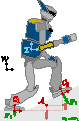
\includegraphics[width=0.5\columnwidth]{Uploaded/Images/framesAndAnchor.pdf} 
\vskip -0.5pc
\caption{representation of the main frames and of the anchor point position computation. $\mathcal{W}$: world frame; $\mathcal{I}$: IMU frame; $\mathcal{C}_{i}$: frame of the $i$-th contact; $\mathcal{A}$: anchor point. In this example, $\boldsymbol{F}_{2} = 2\boldsymbol{F}_{1}$ and so $\lambda_{2} = \frac{2}{3}$.}\label{fig:framesAndAnchor}
\end{center}
\vskip -1.5pc
\end{figure}

Based on this definition, we give the position and linear velocity of the anchor point in the IMU's frame:
\begin{align} 
&{^{\mathcal{I}}}\boldsymbol{p}_{\mathcal{A}} = \sum^{n_{c}}_{i} \lambda_{i}  {^{\mathcal{I}}} \boldsymbol{p}_{{\mathcal{C}}_{i}}, \label{eq:imuAnchorPos} \\
&{^{\mathcal{I}}} \dot{\boldsymbol{p}}_{\mathcal{A}^{\prime}} = \sum^{n_{c}}_{i} \lambda_{i}  {^{\mathcal{I}}} \dot{\boldsymbol{p}}_{{\mathcal{C}}_{i}}, \label{eq:imuAnchorVel}
\end{align} 
with ${^{\mathcal{I}}} \boldsymbol{p}_{{\mathcal{C}}_{i}}$ the position and ${^{\mathcal{I}}} \dot{\boldsymbol{p}}_{{\mathcal{C}}_{i}}$ the linear velocity of the $i$-th contact in the IMU's frame, which are directly provided by the robot's joint encoders and geometrical model.



\section{Tilt Observer with proof of convergence}
The proposed estimator relies on a highly accurate estimate of the IMU's tilt provided by a complementary filter, introduced in~\cite{benallegue2020LyapunovStableOrientationEstimatorHumanoids}, which we will call \emph{Tilt Observer}. 

\subsection{Definition of the State Variables}
The Tilt Observer is able to provide estimates of the following two variables: 
\begin{itemize}
    \item $\boldsymbol{v}_{\mathcal{I}, l} \triangleq \boldsymbol{R}^{T}_{\mathcal{I}} \boldsymbol{v}_{\mathcal{I}} $ the linear velocity of the IMU's frame in the world frame, expressed in the frame of the IMU.
    \item $\boldsymbol{R}^{T}_{\mathcal{I}} \boldsymbol{e}_z$ the tilt of the IMU.
\end{itemize}
We thus define the state variables: 
\begin{alignat}{2}
&\boldsymbol{x}_{1} \triangleq \boldsymbol{v}_{\mathcal{I}, l} \quad &&, \boldsymbol{x}_{1} \in \mathbb{R}^{3}, \label{eq:x1} \\
&\boldsymbol{x}_{2} \triangleq \boldsymbol{R}^{T}_{\mathcal{I}} \boldsymbol{e}_z \quad &&, \boldsymbol{x}_{2} \in \mathbb{S}^{2}. \label{eq:x2}
\end{alignat} 
The set $\mathbb{S}^{2} \subset \mathbb{R}^{3}$ is the unit sphere centered at the origin, and defined as
\begin{equation}
    \mathbb{S}^{2} = \left\{ \boldsymbol{x} \in \mathbb{R}^{3} \vert \lVert \boldsymbol{x} \rVert=1 \right\}
\end{equation}


\subsection{Definition of the Measurements} \label{subsec:tiltMeas}
The measurements required by the Tilt Observer are:
\begin{itemize}
    \item $\boldsymbol{y}_{g}$ the signal of the IMU's gyrometer.
    \item $\boldsymbol{y}_{a}$ the signal of the IMU's accelerometer.
    \item $\boldsymbol{y}_{v}$ a measurement of $\boldsymbol{v}_{\mathcal{I}, l}$.
\end{itemize}
Since no sensor provides a direct measurement of $\boldsymbol{v}_{\mathcal{I}, l}$, we obtain $\boldsymbol{y}_{v}$ from an intermediate zero-velocity pseudo-measurement of the anchor point $\mathcal{A}$ in the world, giving:
\begin{equation}
    \boldsymbol{y}_v = - \left[\boldsymbol{y}_{g}\right]_{\times} {^{\mathcal{I}}}\boldsymbol{p}_{\mathcal{A}} - {^{\mathcal{I}}} \dot{\boldsymbol{p}}_{\mathcal{A}} \label{eq:yv}
\end{equation}
${^{\mathcal{I}}}\boldsymbol{p}_{\mathcal{A}}$ and ${^{\mathcal{I}}} \dot{\boldsymbol{p}}_{\mathcal{A}}$ are the position and linear velocity of the anchor point in the IMU's frame, obtained using\eqref{eq:imuAnchorPos} and \eqref{eq:imuAnchorVel}.

\subsection{Definition of the Filter}
The state dynamics of our system can be written:
\begin{align} 
&\dot{\boldsymbol{x}}_{1} = -\left[\boldsymbol{y}_{g}\right]_{\times} \boldsymbol{x}_{1} - g_{0}\boldsymbol{x}_{2} + \boldsymbol{y}_{a} , \label{eq:x1_dot} \\
&\dot{\boldsymbol{x}}_{2} = -\left[\boldsymbol{y}_{g}\right]_{\times} \boldsymbol{x}_{2}. \label{eq:x2_dot}
\end{align} 
We can then write a complementary filter which uses the system's dynamics as a feed-forward, and corrects the estimated state using the velocity measurement $\boldsymbol{y}_{v}$:
\begin{align} 
& \dot{\hat{\boldsymbol{x}}}_{1}  = - \left[\boldsymbol{y}_{g}\right]_{\times}\hat{\boldsymbol{x}}_{1} - g_{0} \hat{\boldsymbol{x}}_{2}^{\prime} + \boldsymbol{y}_{a} + \alpha_{1} \left(\boldsymbol{y}_{v} - \hat{\boldsymbol{x}}_{1}\right), \label{x1_dot} \\
    & \dot{\hat{\boldsymbol{x}}}_{2}^{\prime} = - \left[\boldsymbol{y}_{g}\right]_{\times} \hat{\boldsymbol{x}}_{2} - \frac{\alpha_{2}}{g_{0}} \left(\boldsymbol{y}_{v} - \hat{\boldsymbol{x}}_{1}\right), \\
    & \dot{\hat{\boldsymbol{x}}}_{2} = - \left[\boldsymbol{y}_{g} - \gamma \left[\hat{\boldsymbol{x}}_{2}\right]_{\times}\hat{\boldsymbol{x}}_{2}^{\prime}\right]_{\times} \hat{\boldsymbol{x}}_{2}.
\end{align} 
$\alpha_1$, $\alpha_2$ and $\gamma$ are positive scalar gains. $\hat{\boldsymbol{x}}_{1} $ and $\hat{\boldsymbol{x}}_{2} $ are estimates of $\boldsymbol{x}_{1} $ and $\boldsymbol{x}_{2} $, respectively. 

The particularity of the Tilt Observer, in comparison to similar complementary filters (e.g.~\cite{martin2016AGlobExpObsVelocityAidedAttitude}), is the use of an intermediate estimate of the tilt, denoted $\hat{\boldsymbol{x}}_{2}^{\prime}$. This intermediate variable allows for a fast convergence of $\hat{\boldsymbol{x}}_{2}$, while making sure it remains on the unit sphere. 


\subsection{Advantages of the Tilt Observer}
The use of a complementary filter for the Tilt Observer presents notable strengths in comparison to other methods like the commonly used Kalman Filter. First, it allows us to work in the frequency domain. This is particularily suitable for our model since the assumption of fixed contacts used to obtain the velocity measurement $\boldsymbol{y}_v$ is more valid in low frequency than in high frequency. In~\eqref{eq:x1_dot}, we thus use the IMU measurements for the high frequency variation of $\hat{\boldsymbol{x}}_{1}$, and $\boldsymbol{y}_v$ for its low frequency variation. Second, one iteration of the filter only consists in computing three equations, it also doesn't involve any matrix inversion and is thus extremely computationally cheap, as will be shown in Section~\ref{subsec:computation_time}. Finally, the formulation as a complementary filter allows to conduct a convergence analysis of the estimation error, providing strong mathematical guarantees on the estimator's performances. Especially here, it has been shown in~\cite{benallegue2020LyapunovStableOrientationEstimatorHumanoids} that:
\begin{itemize}
    \item The dynamics of the estimation error is autonomous, and thus does not depend on the state. 
    \item The intermediate estimator $\left\{\hat{\boldsymbol{x}}_{1}, \hat{\boldsymbol{x}}_{2}^{\prime} \right\}$ is \emph{globally exponentially stable}, with respect to the origin $\left(0,0\right)$.
    \item The full estimator is \emph{almost globally asymptotically stable}, and locally \emph{exponentially stable}.
\end{itemize}

\section{Leg Odometry}

While the tilt of the IMU's frame in the world frame is estimated by the Tilt Observer, its position and yaw are obtained using Leg odometry. Once a contact $i$ is created, its initial pose in the world is obtained by forward kinematics from the current IMU's frame pose and the robot's joint encoders. We call it the contact's \emph{reference} pose $\left\{ \boldsymbol{p}^{\star}_{\mathcal{C}_{i}}, \boldsymbol{R}^{\star}_{\mathcal{C}_{i}}\right\}$, which we consider constant to enforce the contact's anchoring role. This pose is then used to recover the pose of the IMU's frame in the world frame. 
With the proposed pipeline, we thus leverage both the accuracy and mathematical guarantees provided by the Tilt Observer, and the robustness to drift provided by the Leg odometry. Similarly to the computation of the anchor point in Section~\ref{sec:anchor_point}, the contribution of contacts to the Leg odometry is weighted to trust more contacts which are the least prone to slippage, slightly mitigating its effect.


To obtain the yaw from contact information, we compute the weighted average between the reference orientation of the two most reliable contacts\footnote{The two contacts with the highest ratio $u_{i}$ defined in~\eqref{eq:ratio_ui}}. For each contact $i$, we write:
\begin{equation}
    \boldsymbol{R}_{\mathcal{I}, i} = \boldsymbol{R}^{\star}_{\mathcal{C}_{i}} {}^{\mathcal{C}_{i}} \boldsymbol{R}_{\mathcal{I}} 
\end{equation}
We then compute the average $\boldsymbol{R}_{\mathcal{I}, \text{avg}}$ between both contacts using the formalism defined by SO(3) the Lie group of rotation matrices:
\begin{align}
    &\tilde{\boldsymbol{R}} = \boldsymbol{R}^{T}_{\mathcal{I}, 1} \boldsymbol{R}_{\mathcal{I}, 2}  \\
 & \boldsymbol{R}_{\mathcal{I}, \text{avg}} = \boldsymbol{R}_{\mathcal{I}, 1} \text{exp} \left( \lambda_{2} \text{vec}\left(\text{log} \left( \tilde{\boldsymbol{R}}\right)\right)  \right).
\end{align}
exp and log are the \emph{exponential} and \emph{logarithm} maps of SO(3). We note that for small angles, we can use the approximation:
\begin{equation}
log\left(\tilde{\boldsymbol{R}}\right) = \frac{1}{2} \left(\tilde{\boldsymbol{R}}-\tilde{\boldsymbol{R}}^{T}\right), \label{eq:log_small}
\end{equation}
Once the average orientation has been computed, we merge the corresponding yaw with the tilt estimated by the Tilt Observer using the \textcolor{red}{axis agnostic representation} introduced in Section~\ref{sec:axisAgnostic}.

The position of the IMU's frame in the world frame is then obtained from that of the contact reference poses: 
\begin{equation}
    \boldsymbol{p}_{\mathcal{I}} = \sum^{n_{c}}_{i} \lambda_{i} \left( \boldsymbol{p}^{\star}_{{\mathcal{C}}_{i}} - \boldsymbol{R}_{\mathcal{I}} {}^{\mathcal{I}}\boldsymbol{p}_{{\mathcal{C}}_{i}} \right).
\end{equation}
We note that this position is obtained using the IMU's orientation estimate. It thus also benefitiates from the accurate tilt provided by the Tilt Observer.


\section{Experimental Evaluation}
\subsection{Description of the experiments}

The proposed estimator has been evaluated accross two experimental scenarios on two different humanoid robots\footnote{We used the dataset built to evaluate the Kinetics Observer in~\cite{Demont2024KineticsObserver}}:
\begin{itemize}
    \item Experiment 1: A walk on a flat ground over about 18 meters with the robot RHP Friends~\cite{Benallegue2025RhpFriendsJRL}, as shown in Figure~\ref{fig:trajRhps1_3d}. This experiment was repeated 5 times, for a total distance of about 90 meters.
    \item Experiment 2: A multi-contact motion over about 2 meters with the robot HRP-5P~\cite{Kaneko2019Hrp5}. This motion involved an additional contact at the robot's left hand, and non-coplanar contacts on tilted obstacles, as shown in Figure~\ref{fig:hrp5_multicontact}. This experiments was repeated 4 times for a total distance of about 8 meters.
\end{itemize}


\begin{figure}[!t]
\begin{center}
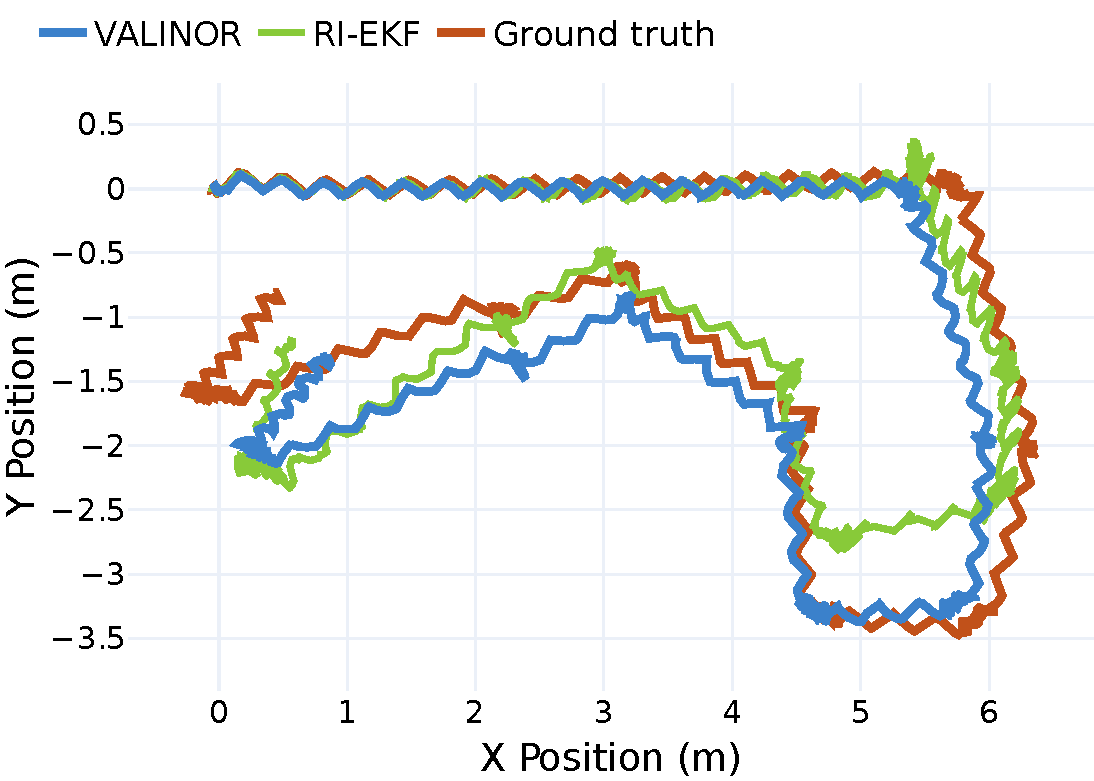
\includegraphics[width=\columnwidth]{Uploaded/Images/trajectory_rhps1.pdf} 
\vskip -0.5pc
\caption{Ground truth and estimated RHP Friend's pelvis trajectory during the first experiment of walk on flat ground.}\label{fig:trajRhps1_3d}
\end{center}
\vskip -1.5pc
\end{figure}

\begin{figure}[!t]
\begin{center}
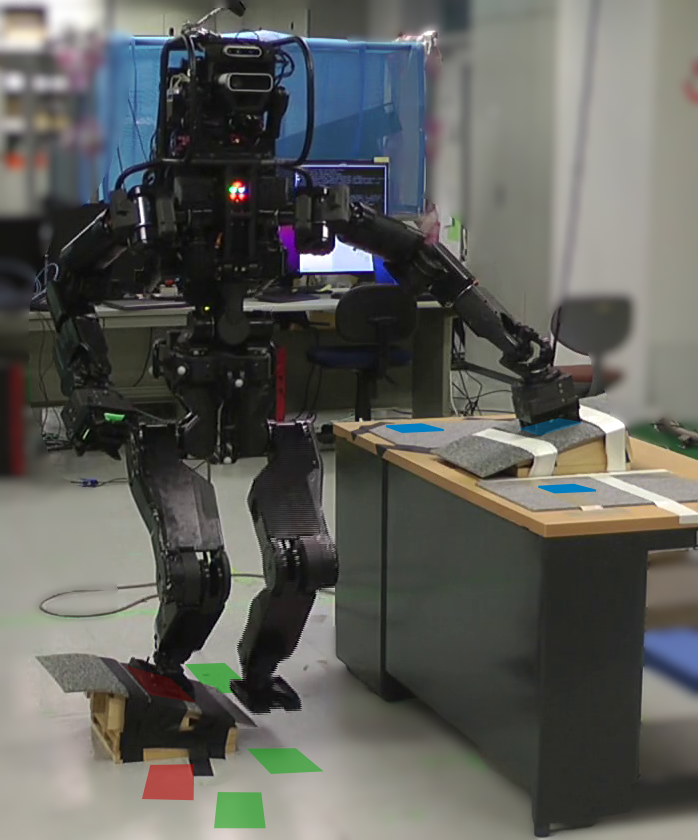
\includegraphics[width=0.6\columnwidth]{Uploaded/Images/multiContactExpe.png} 
\vskip -0.5pc
\caption{Picture of HRP-5P during the multi-contact motion. The imprints of the successive contacts are represented by colored trapezoids: Red: Right foot; Green: Left foot; Blue: Left hand. Figure reused from~\cite{Demont2024KineticsObserver}.}\label{fig:hrp5_multicontact}
\end{center}
\vskip -1.5pc
\end{figure}

\noindent We compare VALINOR, our proposed estimator, with the Right-Invariant EKF (RI-EKF) by~\cite{Hartley2020RIEKF}, on both their computation and their estimation performance. For a fair comparison, both estimators received the same contact state information, from a Schmitt Trigger on the Ground Reaction Force (with thresholds set to 10\% and 15\% of the robot's weight).
Ground truth pose of the robot's pelvis (to which the IMU is fixed on both robots) is provided by a motion capture system (OptiTrack, 16 Prime\textsuperscript{X} with 13 cameras), and its ground truth velocity is obtained by finite differences from the ground truth position then filtered with a zero-phase low-pass filter. The pose of the IMU's frame, estimated by both VALINOR and the RI-EKF, is transformed into that of the pelvis using simple rigid body transformation.

The odometry performance of VALINOR and the RI-EKF is evaluated against the ground truth trajectory using the Relative Error (RE), as defined in~\cite{Zhang2018QuantitativeTrajectoryEvaluation}. RE evaluates the estimation drift over segments of fixed distances. It is particularly relevant for proprioceptive odometry, as it is not affected by global drift, which is unavoidable without exteroceptive sensors. RE therefore provides valuable and easily interpretable insight into the expected local accuracy of the estimator over a given distance.

We compute the Relative Error for lateral ($\boldsymbol{x}, \boldsymbol{y}$) and vertical ($\boldsymbol{z}$) translations separately, since these components are generally influenced by different factors. Accuracy in lateral translation would mainly rely on that of local displacements and of yaw estimation, whereas accuracy in vertical translations would be affected by the accuracy of the estimation of the vertical local displacement, of the tilt, and the reliability of the contact height initialization. Similarily, angular errors in tilt and yaw are also evaluated independently.
The error $e_{l}$ on the tilt estimate is computed with:
\begin{equation}
    e_{l} = \text{arccos}\left(l_{gt}^{T} \hat{l} \right),
\end{equation}
with $l_{gt}$ the ground truth tilt, and $\hat{l}^{T}$ the estimated one.\\
Finally, we also assess the estimation of the IMU's linear velocity in the world. This velocity is expressed in the frame of the IMU such that it is not affected by errors in the orientation estimate. The velocity error is also separated into lateral and vertical components.

\subsection{Experimental Results}

\subsubsection{Computational Performance Evaluation}\label{subsec:computation_time}

To prove the computation speed performance of VALINOR, we compared its average computation time per iteration over the four multi-contact experiments, to that of the RI-EKF. In average, an iteration of VALINOR was computed in 2.547 \textmu s, against 19.315 \textmu s for the RI-EKF. The proposed method is thus more than 7.5 times faster than the state-of-the-art estimator, while proposing \textcolor{red}{equivalent} estimation accuracy, as shown below.

\subsection{Estimation Accuracy Evaluation}

Table~\ref{tab:estimation_eval} regroups the evaluation results of VALINOR's estimation performance compared to those of the RI-EKF during the two experiments on real robots.
The presented errors are computed over all the sequences of each scenario: 5 for the walk on flat ground, and 4 for the multi-contact motion.


\begin{table*}[h] 
\vskip -0.75pc
\setlength{\extrarowheight}{0.6ex}
\addtolength{\tabcolsep}{-0.4em}
\caption{Mean and standard deviation (in parentheses) of the error on the estimations by VALINOR and the RI-EKF, during the two experiments on real robots. The 1 m and the 0.3 m Relative Errors are presented for the walk on flat ground and the multi-contact motion, respectively. The best result for each metric is highlighted in bold.} \label{tab:estimation_eval}
\begin{center}
\vskip -1.25pc
{\footnotesize
    \begin{center}
        \begin{tabu}to\linewidth{| X[c] | X[c] | X[c] | X[c] | X[c] | X[c] | X[c] | X[c] |}
            \hline
            \multicolumn{2}{|c|}{}       &       \multicolumn{2}{c|}{RE Translation [m]}         &    \multicolumn{2}{c|}{RE Orientation [\textdegree] }  &    \multicolumn{2}{c|}{Linear velocity [$\text{m.s}^{-1}$]}     \\     
            \cline{3-8}
            \multicolumn{2}{|c|}{}  &     Lateral    &      Vertical      &   \multirow{2}{*}{Tilt}      &     \multirow{2}{*}{Yaw}    &  Lateral  &  Vertical \\ 
            \multicolumn{2}{|c|}{}  &    \{$\boldsymbol{x}, \boldsymbol{y}$\}    &     $\boldsymbol{z}$      &      &      &   \{$\boldsymbol{x}, \boldsymbol{y}$\}  &  $\boldsymbol{z}$ \\
            
            \tabucline[1.3pt]{-}
            
            \multirow{2}{*}{Walk on}   & VALINOR    &    \textbf{\getErrorResult{Flatodometry}{Tilt}{Relerror}{Transxy}{Meanabs}}  &   \getErrorResult{Flatodometry}{Tilt}{Relerror}{Transz}{Meanabs}   &     \textbf{\getErrorResult{Flatodometry}{Tilt}{Relerror}{Tilt}{Meanabs}}    &     \getErrorResult{Flatodometry}{Tilt}{Relerror}{Yaw}{Meanabs}     &  \getErrorResult{Flatodometry}{Tilt}{Velerror}{EstimateXy}{Meanabs}    &   \textbf{\getErrorResult{Flatodometry}{Tilt}{Velerror}{EstimateZ}{Meanabs}}  \\ 
            & (Proposed)  & (\textbf{\getErrorResult{Flatodometry}{Tilt}{Relerror}{Transxy}{Std}})   &     (\textbf{\getErrorResult{Flatodometry}{Tilt}{Relerror}{Transz}{Std}})   &   (\textbf{\getErrorResult{Flatodometry}{Tilt}{Relerror}{Tilt}{Std}})   &    (\getErrorResult{Flatodometry}{Tilt}{Relerror}{Yaw}{Std})   &  (\getErrorResult{Flatodometry}{Tilt}{Velerror}{EstimateXy}{Std})   &   (\textbf{\getErrorResult{Flatodometry}{Tilt}{Velerror}{EstimateZ}{Std}})  \\ 
            \cline{2-8}
             \multirow{2}{*}{flat ground} &  RI-EKF & \getErrorResult{Flatodometry}{Hartley}{Relerror}{Transxy}{Meanabs}  & \textbf{\getErrorResult{Flatodometry}{Hartley}{Relerror}{Transz}{Meanabs}}      &  \getErrorResult{Flatodometry}{Hartley}{Relerror}{Tilt}{Meanabs}    &    \textbf{\getErrorResult{Flatodometry}{Hartley}{Relerror}{Yaw}{Meanabs}}   &  \textbf{\getErrorResult{Flatodometry}{Hartley}{Velerror}{EstimateXy}{Meanabs}}    &   \getErrorResult{Flatodometry}{Hartley}{Velerror}{EstimateZ}{Meanabs}  \\ 
            &  \cite{Hartley2020RIEKF}  &   (\getErrorResult{Flatodometry}{Hartley}{Relerror}{Transxy}{Std})   &     (\getErrorResult{Flatodometry}{Hartley}{Relerror}{Transz}{Std})    &   (\getErrorResult{Flatodometry}{Hartley}{Relerror}{Tilt}{Std})   &   (\textbf{\getErrorResult{Flatodometry}{Hartley}{Relerror}{Yaw}{Std}})    &  (\textbf{\getErrorResult{Flatodometry}{Hartley}{Velerror}{EstimateXy}{Std}})    &   (\getErrorResult{Flatodometry}{Hartley}{Velerror}{EstimateZ}{Std})  \\ 
            \tabucline[1.3pt]{-}
            \multirow{2}{*}{Multi-contact} &   VALINOR  &  \textbf{\getErrorResult{Multicontact}{Tilt}{Relerror}{Transxy}{Meanabs}}  &  \textbf{\getErrorResult{Multicontact}{Tilt}{Relerror}{Transz}{Meanabs}}   &    \textbf{\getErrorResult{Multicontact}{Tilt}{Relerror}{Tilt}{Meanabs}}    &    \textbf{\getErrorResult{Multicontact}{Tilt}{Relerror}{Yaw}{Meanabs}}     &  \getErrorResult{Multicontact}{Tilt}{Velerror}{EstimateXy}{Meanabs}    &   \textbf{\getErrorResult{Multicontact}{Tilt}{Velerror}{EstimateZ}{Meanabs}}  \\ 
             & (Proposed)  &  (\textbf{\getErrorResult{Multicontact}{Tilt}{Relerror}{Transxy}{Std}})   &      (\textbf{\getErrorResult{Multicontact}{Tilt}{Relerror}{Transz}{Std}})      &   (\textbf{\getErrorResult{Multicontact}{Tilt}{Relerror}{Tilt}{Std}})   &     (\textbf{\getErrorResult{Multicontact}{Tilt}{Relerror}{Yaw}{Std}})   &  (\getErrorResult{Multicontact}{Tilt}{Velerror}{EstimateXy}{Std})   &   (\textbf{\getErrorResult{Multicontact}{Tilt}{Velerror}{EstimateZ}{Std}})  \\ 
            \cline{2-8}     
            \multirow{2}{*}{motion}   & RI-EKF  &  \getErrorResult{Multicontact}{Hartley}{Relerror}{Transxy}{Meanabs}  &   \getErrorResult{Multicontact}{Hartley}{Relerror}{Transz}{Meanabs}   &    \getErrorResult{Multicontact}{Hartley}{Relerror}{Tilt}{Meanabs}    &    \getErrorResult{Multicontact}{Hartley}{Relerror}{Yaw}{Meanabs}   &  \textbf{\getErrorResult{Multicontact}{Hartley}{Velerror}{EstimateXy}{Meanabs}}    &   \getErrorResult{Multicontact}{Hartley}{Velerror}{EstimateZ}{Meanabs}  \\ 
            & \cite{Hartley2020RIEKF} & (\getErrorResult{Multicontact}{Hartley}{Relerror}{Transxy}{Std})    &     (\getErrorResult{Multicontact}{Hartley}{Relerror}{Transz}{Std})    &     (\getErrorResult{Multicontact}{Hartley}{Relerror}{Tilt}{Std})   &    (\getErrorResult{Multicontact}{Hartley}{Relerror}{Yaw}{Std})    &  (\textbf{\getErrorResult{Multicontact}{Hartley}{Velerror}{EstimateXy}{Std}})    &   (\getErrorResult{Multicontact}{Hartley}{Velerror}{EstimateZ}{Std})  \\ 
            \hline     
        \end{tabu}
    \end{center}
}
\end{center}
\vskip -0.25pc
\end{table*}


We first note that the relative strengths of both estimators were consistent accross both experiments, and that overall, they both displayed satisfactory estimation performance. Indeed, without the use of any exteroceptive sensors, their errors in translation estimates remain of the order of the centimer per meter walked, those on orientation estimates remain around 1\textdegree \ per meter walked, and finally their error in velocity estimates remain below 2 cm.s$^{-1}$. Now we give more insights in the obtained results:
\begin{itemize}
    \item VALINOR estimated more accurately lateral translations, improving the estimation by over 30\% and 40\% compared to the RI-EKF. Additionally, it improved the estimation of the tilt by about 28\% in Experiment 1 and by 60\% in Experiment 2, reaching an average error of only 0.23\textdegree. For both translations and tilt estimates, our method displayed a significantly lower standard deviation of the error, proving an improved estimation consistency. 
    \item The RI-EKF estimated lateral velocities more accurately than VALINOR, with an improvement of about 20\% of the error.\textcolor{red}{Dire ca?}
    \item Both estimators showed similar performance for the estimation of the yaw and of vertical translation and velocity.
\end{itemize}

Concerning vertical translations, we noticed that both estimators drifted upwards during the walk on flat ground, which involved longer walks and many more steps than the multi-contact motion. One of the reasons, inherent to Leg odometry, is its reliance on the quality of the contact detection. For example, detecting contacts consistently too early (when they are not perfectly still yet), would cause the estimate to drift on each step. Conversely, drift can also occur when detecting contacts consistently too late, due to the robot's structural deformation under the contact force, etc. While investigating, we could indeed reduce the vertical drift by tuning the thresholds of the Schmitt Trigger used for contact detection. However, we decided to leave them changed to ensure a fair comparison. The other main factor explaining the vertical drift is the quality of the pitch estimate, which significantly affects vertical translation estimates during long forward walks. Especially during the first part of the walk on flat ground\textcolor{red}{maybe add plot of pitch and vertical translation, and in that case use the time interval directly}, the RI-EKF estimated the IMU's pitch with an ``offset'' of about 1.5\textdegree, which made its estimated vertical translation quickly drift downwards\footnote{This result was already observed and detailed in~\cite{Demont2024KineticsObserver}.}.
The pitch estimation error then becomes negative, making the robot drift back upwards. This phenomenon, observed during the five trials of first experiment, notably explains the high standard deviation of the vertical translation error by the RI-EKF.

\textcolor{red}{Conclure ici?}

\section{CONCLUSION}

This paper proposes a lightweight estimator for humanoid robots. It combines Leg odometry with the Tilt Observer, which provides at high frequency an accurate and reliable estimate of the robot's tilt and linear velocity. Our experimental results, obtained on real humanoid robots, show that VALINOR achieves accuracy equivalent to the state of the art, while being 7.5 times faster. Further work would aim at improving the coupling between the Inertial and the Leg odometry, notably such that the position and yaw estimates leverage better IMU measurements. Other extensions could investigate the incorporation of other sensors into the framework.



\section*{DECLARATIONS}
\subsection*{Funding }
This paper is based on results obtained from a project of Programs for Bridging the gap between R\&D and the IDeal society (society 5.0) and Generating Economic and social value (BRIDGE)/Practical Global Research in the AI x Robotics Services, implemented by the Cabinet Office, Government of Japan, and partially funded by the Japan Science and Technology Agency (JST) with the JST-Mirai Program, grant number JPMJMI21H4.


% \bibliographystyle{IJCAS}
% \bibliography{Uploaded/Bibliography}

\bibliographystyle{IEEEtran}
\bibliography{IEEEabrv, Uploaded/Bibliography}

% \biography{Uploaded/Arnaud.png}{Arnaud Demont}{received the M.S. degree in mechanical engineering with a specialization in mechatronics and systems from the National Institute of Applied Sciences of Lyon, France, and a second M.S. degree in automation and robotics in intelligent systems from the University of  Technology of Compiègne, France, in 2021 and 2023 respectively. He is currently pursuing the PhD degree of the Université Paris-Saclay, France, within the CRNS-AIST Joint Robotics Laboratory in Tsukuba, Japan. His research interests include state estimation for legged robots, multi-sensor fusion, and mobile robot perception and autonomous navigation.
% }

% \biography{Uploaded/Mehdi.png}{Mehdi Benallegue}{holds an engineering degree from the National Institute of Computer Science (INI) in Algeria, obtained in 2007. He earned a master's degree from the University of Paris 7, France, in 2008, and a Ph.D. from the University of Montpellier 2, France, in 2011. His research took him to the Franco-Japanese Robotics Laboratory in Tsukuba, Japan, and to INRIA Grenoble, France. He also worked as a postdoctoral researcher at the Collège de France and at LAAS CNRS in Toulouse, France. Currently, he is a Research Associate with CNRS AIST Joint robotics Laboratory in Tsukuba, Japan. His research interests include robot estimation and control, legged locomotion, biomechanics, neuroscience, and computational geometry.
% }

% \biography{Uploaded/Aziz.png}{Prof. Abdelaziz Benallegue}{received the B.S. degree in electronics engineering from Algiers National Polytechnic School, Algeria in 1986 and both the M.S. and Ph.D. degrees in automatic control and robotics from University of Pierre and Marie Curie, Paris 6 (currently Sorbonne University), France in 1987 and 1991 respectively. He was Associate professor in Automatic Control and Robotics at the University Pierre et Marie Curie, Paris 6 (currently Sorbonne University) from 1992 to 2002. In September 2002, he joined the University of Versailles St Quentin as full Professor assigned. He was a CNRS delegate at JRL-AIST, Japan for three years, between 2016 and 2022. His research activities are mainly related to linear and non-linear estimation and control theory (adaptive control, robust control, neural learning control, observers, multi-sensor fusion, etc.) with applications in robotics (humanoid robots, aerial robots, manipulator robots, etc.).
% }

\clearafterbiography
\relax 

\end{document}

